\documentclass[12pt]{article}
\usepackage[utf8]{inputenc}
\usepackage[T1]{fontenc}
\usepackage{amsmath}
\usepackage{amsfonts}
\usepackage{amssymb}
\usepackage[version=4]{mhchem}
\usepackage{stmaryrd}
\usepackage{graphicx}
\usepackage{physics}

\usepackage{listings} % Required for insertion of code
\usepackage{xcolor} % Required for custom colors

% Define custom colors
\definecolor{codegreen}{rgb}{0,0.6,0}
\definecolor{codegray}{rgb}{0.5,0.5,0.5}
\definecolor{codepurple}{rgb}{0.58,0,0.82}
\definecolor{backcolour}{rgb}{0.95,0.95,0.92}

% Setup the style for code listings
\lstdefinestyle{mystyle}{
    backgroundcolor=\color{backcolour},   
    commentstyle=\color{codegreen},
    keywordstyle=\color{magenta},
    numberstyle=\tiny\color{codegray},
    stringstyle=\color{codepurple},
    basicstyle=\ttfamily\footnotesize,
    breakatwhitespace=false,         
    breaklines=true,                 
    captionpos=b,                    
    keepspaces=true,                 
    numbers=left,                    
    numbersep=5pt,                  
    showspaces=false,                
    showstringspaces=false,
    showtabs=false,                  
    tabsize=2
}

% Activate the style
\lstset{style=mystyle}


\title{PROBLEMS: }

\author{}
\date{}


\begin{document}
\maketitle
Physics $125 \mathrm{~b}$

Problem set number 7

Due midnight Wednesday, February 21, 2024

READING: Pages 592-607 in Shankar on Berry's phase.
\section{}
\begin{enumerate}
  \setcounter{enumi}{24}
  \item Let's continue a bit further with the dipole interaction of problem 24. You obtained, I hope, an expression for the "electric dipole Hamiltonian". But it might look a bit mysterious. If this really describes an electric dipole interaction with a uniform external field, we might expect the Hamiltonian to look something like
\end{enumerate}


\begin{equation*}
H_{D}^{\prime}=-q E Z \sin \omega t . \tag{1}
\end{equation*}


That is, $q Z$ looks like a dipole moment. Consider the expectation value $\left\langle n\left|P_{z}\right| 0\right\rangle$ with respect to two eigenstates of $H_{0}$. Show that this can be written in terms of an expectation value $\langle n|Z| 0\rangle$ and quantities such as the electron mass, $m$, and the energy difference between the states. Rewrite $H_{D}$ using this relation. Does it look more intuitive now?
\subsection{}
We want to consider the commutator between $H_0$ and $Z$. For the original Hamiltonian, we had the 
\begin{equation}
  H_{0}=\frac{P^{2}}{2m}+V(R)
\end{equation}
Since the potential only has a radial dependence, which means it only depends on $R$, and we know that $Z$ commutes with each of the Cartesian coordinates, we can say that $[V(R),Z]=0$.
We can expand the total momentum operator squared into its individual Cartesian components
\begin{equation}
  P^{2}=P_{x}^{2}+P_{y}^{2}+P_{z}^{2}
\end{equation}
Because the $Z$ operator commutes with the $P_{x}$ and $P_{y}$ operators, we have found that the commutator $[H_0,Z]$ is the same as $\frac{1}{2m}[P_{z}^{2},Z]$. Then, we know that:
\begin{equation}
  [P_{z}^{2},Z]=P_{z}[P_{z},Z]+[P_{z},Z]P_{z}
\end{equation}
and we can use the commutator $[P_{z},Z]=i\hbar$ to get:
\begin{equation}
  [P_{z}^{2},Z]=i\hbar P_{z}+i\hbar P_{z}=2i\hbar P_{z} \rightarrow [H_0,Z]=\frac{i\hbar}{m} P_{z}
\end{equation}
So now that us consider the virginal expectation value:
\begin{equation}
  \left\langle n\left|P_{z}\right| 0\right\rangle
\end{equation}
We can use the commutator to get:
\begin{equation}
  \left\langle n\left|P_{z}\right| 0\right\rangle = \frac{m}{i\hbar}\left\langle n\left|[H_0,Z\right]| 0\right\rangle
\end{equation}
Expanding the commutator gives:
\begin{equation}
  \left\langle n\left|P_{z}\right| 0\right\rangle = \frac{m}{i\hbar}\left\langle n\left|H_0Z-ZH_0\right| 0\right\rangle = \frac{m}{i\hbar}\left\langle n\left|H_0Z\right| 0\right\rangle - \frac{m}{i\hbar}\left\langle n\left|ZH_0\right| 0\right\rangle
\end{equation}
Let us call the unpertirbed energies of $|n\rangle$ and $|0\rangle$ $E_n$ and $E_0$ respectively. All of these entities are real, so:
\begin{equation}
  = \frac{m}{i\hbar}\left(E_n\left\langle n\left|Z\right| 0\right\rangle - E_0\left\langle n\left|Z\right| 0\right\rangle\right) = \frac{m}{i\hbar}\left(E_n-E_0\right)\left\langle n\left|Z\right| 0\right\rangle
\end{equation}
Now, the expectation value of the dipole antonian between the final and initial states is given by:
\begin{equation}
  \left\langle n\left|H_{D}\right| 0\right\rangle = -qE\sin(\omega t)\left\langle n\left|Z\right| 0\right\rangle
\end{equation}
The matrix element of the $Z$ operator between the final and initial states in terms of the expectation value of the momentum operator is:
\begin{equation}
  \left\langle n\left|Z\right| 0\right\rangle = \frac{i\hbar}{m(E_n-E_0)}\left\langle n\left|P_{z}\right| 0\right\rangle
\end{equation}
So we can rewrite the dipole Hamiltonian as:
\begin{equation}
  \left\langle n\left|H_{D}\right| 0\right\rangle = -qE\sin(\omega t)\frac{i\hbar}{m(E_n-E_0)}\left\langle n\left|P_{z}\right| 0\right\rangle
\end{equation}
So without the expectation value, I got:
\begin{equation}
  H_{D}=-qE\sin(\omega t)\frac{i\hbar}{m(E_n-E_0)}P_{z}
\end{equation}
The original Hamiltonian for the electronic dipole was more intuitive as two charges separated by a distance $Z$ and then interacting with an electric field $E$. In this problem, we got something in terms of the momentum operator, which is not as intuitive as what was said previously.
\section{}
\begin{enumerate}
  \setcounter{enumi}{25}
  \item When we continue to apply our dipole approximation to an atom, we'll find that the dipole operator produces transitions from the ground state $|0\rangle$ to other eigenstates, $|n\rangle$, of $H_{0}$. The relative strengths of these transitions is given by an "oscillator strength":
\end{enumerate}


\begin{equation*}
f_{n 0}=2 m \omega_{n 0}|\langle n|Z| 0\rangle|^{2}, \tag{2}
\end{equation*}


where $\omega_{n 0}=E_{n}-E_{0}$ is the energy difference between the states. Note that $f_{n 0}$ is dimensionless. Demonstrate the oscillator strength "sum rule":


\begin{equation*}
\sum_{n} f_{n 0}=1 \tag{3}
\end{equation*}


The work you have done in problem 25 will likely come in handy here.
\subsection{}
That us only substitute the relation that we god for the expectation value of $Z$ in terms of the momentum operator only for one of the terms in the square:
\begin{equation}
  f_{n 0}=2 m \omega_{n 0}\left(\frac{1}{2}\langle n|Z| 0\rangle \frac{i\hbar}{m(E_n-E_0)}\left\langle 0\left|P_{z}\right| n\right\rangle - \frac{1}{2}\langle n|P_{z}| 0\rangle \frac{i\hbar}{m(E_n-E_0)}\left\langle 0\left|Z\right| n\right\rangle\right)
\end{equation}
We note that in one of the terms the complex number was congregated, so we have two reverse the sign of one of these.\\
Making a lot of cancellations including for the mass, for $\omega _{n0}= E_n-E_0$ and factoring out the term of $i\hbar$ gives:
\begin{equation}
  f_{n 0}=i\hbar\left(\langle n|[Z,P_z]| 0\rangle\right)
\end{equation}
Then, we also know that $[Z,P_z]=-i\hbar$, so we get:
\begin{equation}
  f_{n 0}=- i\hbar i\hbar \langle n|| 0\rangle
\end{equation}
When we consider the whole sum, only one of these terms will survive from Arthur normality, so we get:
\begin{equation}
  \sum_{n} f_{n 0}=-i\hbar i\hbar \sum_{n}\langle n|| 0\rangle = -i\hbar i\hbar = \hbar^2
\end{equation}
But we have that $\hbar = 1$, so we get:
\begin{equation}
  \sum_{n} f_{n 0}=1
\end{equation}

\section{}
\begin{enumerate}
  \setcounter{enumi}{26}
  \item We discussed Berry's phase in class, including the example of the Aharonov-Bohm effect. Let us try another example.
\end{enumerate}

Consider a spin- $1 / 2$ particle of magnetic moment $\mu$ in a magnetic field, $\mathbf{B}$. Let the strength of the magnetic field be a constant, but suppose that its direction is slowly changing. Suppose the magnetic field vector is swept through a closed curve (i.e., think of the tip of its vector as being varied along a closed curve on the surface of a sphere). Thus, two parameters describing the direction of the field are being varied, which we might take to be the polar angles $(\theta, \phi)$.

(a) What does "slow" mean? That is, on what time scale should the variation be slow, in order for the adiabatic approximation to be reasonable?
\subsection{}
This is a two state system with two energies:
\begin{equation}
  E_{\pm}=\pm \mu B
\end{equation}
The magnitude of the energy difference is:
\begin{equation}
  \Delta = 2\mu B
\end{equation}
We have the following condition from the nodes:
\begin{figure}
  \centering
  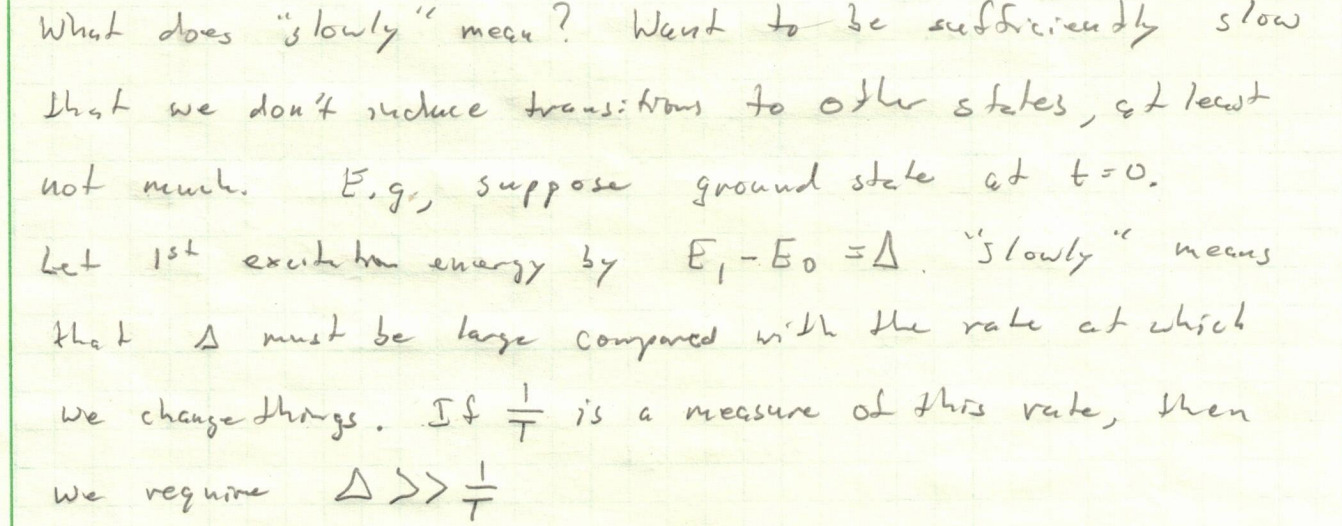
\includegraphics[scale=0.5]{adiabatic.png}
\end{figure}
So, our condition is:
\begin{equation}
  \Delta  \gg \frac{1}{T}
\end{equation}
Alternatively, we have:
\begin{equation}
  T \gg \frac{1}{2\mu B}
\end{equation}

(b) What is the expectation value of the spin vector in the adiabatic ground state?
\subsection{}

(c) Express the adiabatic ground state wave function, $\psi_{\theta \phi}^{(0)}$, in terms of the adiabaticallyvaried parameters. You can in principle achieve this from your result to part (b), but it will probably be easier to accomplish by performing a rotation on a vector to the desired polar angles. The text pages 329-333 discuss finite rotations. The discussion of spin-1/2 in Chapter 14 of the text may also be helpful. I have also uploaded to module 7 the supplementary note on angular momentum from $\mathrm{Ph} 125$ a.

(d) Suppose we let the $\mathbf{B}$ field direction rotate slowly around the 3-axis at constant $\theta$. Calculate Berry's phase for this situation. [Recall that Berry's phase is the change in the phase of the adiabatic wave function (ground state here) over one complete circuit in parameter space. We found that the Berry phase is given by:


\begin{equation*}
\gamma_{B}=i \oint d \boldsymbol{\alpha} \cdot\left\langle\psi_{\boldsymbol{\alpha}}^{(0)} \mid \nabla_{\boldsymbol{\alpha}} \psi_{\boldsymbol{\alpha}}^{(0)}\right\rangle \tag{4}
\end{equation*}


where $\boldsymbol{\alpha}$ is a vector in parameter space.] See if you can give a geometric interpretation to your answer, in terms of an amount of solid angle swept out by the circuit in parameter space.
\section{}
\begin{enumerate}
  \setcounter{enumi}{27}
  \item Let us investigate our quantum electromagnetic field operators and in particular think about a notion for the energy density in the vacuum. We defined the quantum mechanical electromagnetic field operators $\hat{A}_{\mathrm{k}} \boldsymbol{\epsilon}$ and $\hat{A}_{\mathrm{k} \boldsymbol{\epsilon}}^{\dagger}$ :
\end{enumerate}


\begin{align*}
& \hat{A}_{\mathbf{k} \epsilon}\left|N_{\mathbf{k}_{1} \epsilon_{1}}, \ldots, N_{\mathbf{k} \epsilon}, \ldots\right\rangle=\sqrt{\frac{2 \pi}{\omega}} \sqrt{N_{\mathbf{k} \epsilon}}\left|N_{\mathbf{k}_{1} \epsilon_{1}}, \ldots, N_{\mathbf{k} \epsilon}-1, \ldots\right\rangle  \tag{5}\\
& \hat{A}_{\mathbf{k} \epsilon}^{\dagger}\left|N_{\mathbf{k}_{1} \epsilon_{1}}, \ldots, N_{\mathbf{k} \epsilon}, \ldots\right\rangle=\sqrt{\frac{2 \pi}{\omega}} \sqrt{N_{\mathbf{k} \epsilon}+1}\left|N_{\mathbf{k}_{1} \epsilon_{1}}, \ldots, N_{\mathbf{k} \epsilon}+1, \ldots\right\rangle . \tag{6}
\end{align*}


(a) Determine the commutation relations among these operators.
\subsection{}
We want to compute 3 commutation relations:
\begin{equation}
  [\hat{A}_{\mathbf{k} \epsilon},\hat{A}_{\mathbf{k^{\prime}} \epsilon^{\prime}}] = \hat{A}_{\mathbf{k} \epsilon}\hat{A}_{\mathbf{k^{\prime}} \epsilon^{\prime}} - \hat{A}_{\mathbf{k^{\prime}} \epsilon^{\prime}}\hat{A}_{\mathbf{k} \epsilon}
\end{equation}
We want to consider the effect of this on the arbor every state like $\ket{\cdots ,N_{\mathbf{k} \epsilon}, \cdots, N_{\mathbf{k^{\prime}} \epsilon^{\prime}}, \cdots}$.
\begin{equation}
\hat{A}_{\mathbf{k} \epsilon}\sqrt{\frac{2\pi}{\omega }} \sqrt{N_{\mathbf{k^{^{\prime}}\epsilon^{\prime}}}}\ket{\cdots ,N_{\mathbf{k} \epsilon}, \cdots, N_{\mathbf{k^{\prime}} \epsilon^{\prime}}-1, \cdots} - \hat{A}_{\mathbf{k^{\prime}} \epsilon^{\prime}}\sqrt{\frac{2\pi}{\omega }} \sqrt{N_{\mathbf{k} \epsilon}}\ket{\cdots ,N_{\mathbf{k} \epsilon}-1, \cdots, N_{\mathbf{k^{\prime}} \epsilon^{\prime}}, \cdots}
\end{equation}
Applying the second operator gives:
\begin{equation}
  \sqrt{\frac{2\pi}{\omega }} \sqrt{N_{\mathbf{k^{^{\prime}}\epsilon^{\prime}}}}\sqrt{\frac{2\pi}{\omega }} \sqrt{N_{\mathbf{k} \epsilon}}\ket{\cdots ,N_{\mathbf{k} \epsilon}-1, \cdots, N_{\mathbf{k^{\prime}} \epsilon^{\prime}}-1, \cdots} - \sqrt{\frac{2\pi}{\omega }} \sqrt{N_{\mathbf{k} \epsilon}}\sqrt{\frac{2\pi}{\omega }} \sqrt{N_{\mathbf{k^{^{\prime}}\epsilon^{\prime}}}}\ket{\cdots ,N_{\mathbf{k^{^{\prime}}\epsilon^{\prime}}}-1, \cdots, N_{\mathbf{k} \epsilon}-1, \cdots}
\end{equation}
We can factor out the constants:
\begin{equation}
  = \frac{2\pi}{\omega } \sqrt{N_{\mathbf{k^{^{\prime}}\epsilon^{\prime}}}}\sqrt{N_{\mathbf{k} \epsilon}}\left( \ket{\cdots ,N_{\mathbf{k} \epsilon}-1, \cdots, N_{\mathbf{k^{\prime}} \epsilon^{\prime}}-1, \cdots} - \ket{\cdots ,N_{\mathbf{k^{^{\prime}}\epsilon^{\prime}}}-1, \cdots, N_{\mathbf{k} \epsilon}-1, \cdots}\right) = 0
\end{equation}
Let us also consider the case of $\mathbf{k},\epsilon = \mathbf{k^{\prime}},\epsilon^{\prime}$:
\begin{equation}
  [\hat{A}_{\mathbf{k} \epsilon},\hat{A}_{\mathbf{k} \epsilon}] = \hat{A}_{\mathbf{k} \epsilon}\hat{A}_{\mathbf{k} \epsilon} - \hat{A}_{\mathbf{k} \epsilon}\hat{A}_{\mathbf{k} \epsilon} = 0
\end{equation}
So, this case is trivially 0.\\
\begin{equation}
  [\hat{A}_{\mathbf{k} \epsilon}^{\dagger},\hat{A}_{\mathbf{k^{\prime}} \epsilon^{\prime}}^{\dagger}]
\end{equation}
By symmetry, this is also 0.\\
\begin{equation}
  [\hat{A}_{\mathbf{k} \epsilon},\hat{A}^\dagger_{\mathbf{k^{\prime}} \epsilon^{\prime}}] = \hat{A}_{\mathbf{k} \epsilon}\hat{A}^\dagger_{\mathbf{k^{\prime}} \epsilon^{\prime}} - \hat{A}^\dagger_{\mathbf{k^{\prime}} \epsilon^{\prime}}\hat{A}_{\mathbf{k} \epsilon}
\end{equation}
Apply this to the state $\ket{\cdots ,N_{\mathbf{k} \epsilon}, \cdots, N_{\mathbf{k^{\prime}} \epsilon^{\prime}}, \cdots}$:
\begin{equation}
  \hat{A}_{\mathbf{k} \epsilon}\sqrt{\frac{2\pi}{\omega }} \sqrt{N_{\mathbf{k^{^{\prime}}\epsilon^{\prime}}}+1}\ket{\cdots ,N_{\mathbf{k} \epsilon}, \cdots, N_{\mathbf{k^{\prime}} \epsilon^{\prime}}+1, \cdots} - \hat{A}^\dagger_{\mathbf{k^{\prime}} \epsilon^{\prime}}\sqrt{\frac{2\pi}{\omega }} \sqrt{N_{\mathbf{k} \epsilon}}\ket{\cdots ,N_{\mathbf{k} \epsilon}-1, \cdots, N_{\mathbf{k^{\prime}} \epsilon^{\prime}}, \cdots}
\end{equation}
Applying the second operator gives:
\begin{equation}
  =\sqrt{\frac{2\pi}{\omega }} \sqrt{N_{\mathbf{k^{^{\prime}}\epsilon^{\prime}}}+1}\sqrt{\frac{2\pi}{\omega }} \sqrt{N_{\mathbf{k} \epsilon}}\ket{\cdots ,N_{\mathbf{k} \epsilon}-1, \cdots, N_{\mathbf{k^{\prime}} \epsilon^{\prime}}+1, \cdots}
\end{equation}
\begin{equation}
  - \sqrt{\frac{2\pi}{\omega }} \sqrt{N_{\mathbf{k} \epsilon}}\sqrt{\frac{2\pi}{\omega }} \sqrt{N_{\mathbf{k^{^{\prime}}\epsilon^{\prime}}}+1}\ket{\cdots ,N_{\mathbf{k} \epsilon}-1, \cdots, N_{\mathbf{k^{\prime}} \epsilon^{\prime}}+1, \cdots}
\end{equation}
We can factor out the constants:
\begin{equation}
  = \frac{2\pi}{\omega } \sqrt{N_{\mathbf{k^{^{\prime}}\epsilon^{\prime}}}+1}\sqrt{N_{\mathbf{k} \epsilon}}\left( \ket{\cdots ,N_{\mathbf{k} \epsilon}-1, \cdots, N_{\mathbf{k^{\prime}} \epsilon^{\prime}}+1, \cdots} - \ket{\cdots ,N_{\mathbf{k} \epsilon}-1, \cdots, N_{\mathbf{k^{\prime}} \epsilon^{\prime}}+1, \cdots}\right) = 0
\end{equation}
Now, we consider the case of $\mathbf{k},\epsilon = \mathbf{k^{\prime}},\epsilon^{\prime}$:
\begin{equation}
  [\hat{A}_{\mathbf{k} \epsilon},\hat{A}^\dagger_{\mathbf{k} \epsilon}] = \hat{A}_{\mathbf{k} \epsilon}\hat{A}^\dagger_{\mathbf{k} \epsilon} - \hat{A}^\dagger_{\mathbf{k} \epsilon}\hat{A}_{\mathbf{k} \epsilon}
\end{equation}
Apply this to the state $\ket{\cdots ,N_{\mathbf{k} \epsilon}, \cdots}$:
\begin{equation}
  \hat{A}_{\mathbf{k} \epsilon}\sqrt{\frac{2\pi}{\omega }} \sqrt{N_{\mathbf{k} \epsilon}+1}\ket{\cdots ,N_{\mathbf{k} \epsilon}+1, \cdots} - \hat{A}^\dagger_{\mathbf{k} \epsilon}\sqrt{\frac{2\pi}{\omega }} \sqrt{N_{\mathbf{k} \epsilon}}\ket{\cdots ,N_{\mathbf{k} \epsilon}-1, \cdots}
\end{equation}
Applying the second operator gives:
\begin{equation}
  =\sqrt{\frac{2\pi}{\omega }} \sqrt{N_{\mathbf{k} \epsilon}+1}\sqrt{\frac{2\pi}{\omega }} \sqrt{N_{\mathbf{k} \epsilon}+1}\ket{\cdots ,N_{\mathbf{k} \epsilon}, \cdots}  - \sqrt{\frac{2\pi}{\omega }} \sqrt{N_{\mathbf{k} \epsilon}}\sqrt{\frac{2\pi}{\omega }} \sqrt{N_{\mathbf{k} \epsilon}}\ket{\cdots ,N_{\mathbf{k} \epsilon}, \cdots}
\end{equation}
We can factor out the constants:
\begin{equation}
  = \frac{2\pi}{\omega } \left( \left( N_{\mathbf{k} \epsilon}+1\right) - N_{\mathbf{k} \epsilon}\right)\ket{\cdots ,N_{\mathbf{k} \epsilon}, \cdots} = \frac{2\pi}{\omega }\ket{\cdots ,N_{\mathbf{k} \epsilon}, \cdots}
\end{equation}
So, we have that:
\begin{equation}
  [\hat{A}_{\mathbf{k} \epsilon},\hat{A}^\dagger_{\mathbf{k} \epsilon}] = \frac{2\pi}{\omega }
\end{equation}
and thus we have a relation involving the kronecker delta for this one:
\begin{equation}
  [\hat{A}_{\mathbf{k} \epsilon},\hat{A}^\dagger_{\mathbf{k^{\prime}} \epsilon^{\prime}}] = \frac{2\pi}{\omega }\delta_{\mathbf{k}\mathbf{k^{\prime}}}\delta_{\epsilon\epsilon^{\prime}}
\end{equation}

(b) We may define the quantum mechanical electric field operator according to:


\begin{equation*}
\hat{\mathbf{E}}(\mathbf{x})=\frac{1}{\sqrt{V}} \sum_{\mathbf{k} \boldsymbol{\epsilon}}\left(-i \omega \hat{A}_{\mathbf{k} \boldsymbol{\epsilon}} \boldsymbol{\epsilon} e^{i \mathbf{k} \cdot \mathbf{x}}+i \omega \hat{A}_{\mathbf{k} \boldsymbol{\epsilon}}^{\dagger} \boldsymbol{\epsilon}^{*} e^{-i \mathbf{k} \cdot \mathbf{x}}\right) . \tag{7}
\end{equation*}


Make sure this definition makes sense to you. We know that classically we can compute the energy density in an electromagnetic field as proportional to the squared electric (plus squared magnetic) fields. Compute the expectation value:


\begin{equation*}
\left\langle\Omega\left|\hat{\mathbf{E}}(\mathbf{x}) \cdot \hat{\mathbf{E}}\left(\mathbf{x}^{\prime}\right)\right| \Omega\right\rangle \tag{8}
\end{equation*}


Try to express your answer in terms of a dimensionless integral in one dimension (which will perhaps look divergent). Make sure the dimension of the coefficient is what you expect.

(c) Now let's consider the average, $\hat{\overline{\mathbf{E}}}(\mathbf{x})$, of $\hat{\mathbf{E}}(\mathbf{x})$ over a small volume $\mathcal{V}$. That is, we are interested in the average energy density in a small volume. What is


\begin{equation*}
\left\langle\Omega\left|[\hat{\overline{\mathbf{E}}}(\mathbf{x})]^{2}\right| \Omega\right\rangle, \tag{9}
\end{equation*}


and what happens as $\mathcal{V} \rightarrow 0$ ? You may wish to think about your result in terms of harmonic oscillators and zero point energies.
\subsection{}
The average of the electric field over a small volume $\mathcal{V}$ is given by:
\begin{equation}
  \hat{\overline{\mathbf{E}}}(\mathbf{x})=\mathcal{V}^{-3/2}\sum_{\mathbf{k} \boldsymbol{\epsilon}}\left(-i \omega \hat{A}_{\mathbf{k} \boldsymbol{\epsilon}} \boldsymbol{\epsilon} e^{i \mathbf{k} \cdot \mathbf{x}}+i \omega \hat{A}_{\mathbf{k} \boldsymbol{\epsilon}}^{\dagger} \boldsymbol{\epsilon}^{*} e^{-i \mathbf{k} \cdot \mathbf{x}}\right)
\end{equation}
so the square of this relation is:
\begin{equation}
  (\hat{\overline{\mathbf{E}}}(\mathbf{x}))^2=\mathcal{V}^{-3}\sum_{\mathbf{k} \boldsymbol{\epsilon}}\left(-i \omega \hat{A}_{\mathbf{k} \boldsymbol{\epsilon}} \boldsymbol{\epsilon} e^{i \mathbf{k} \cdot \mathbf{x}}+i \omega \hat{A}_{\mathbf{k} \boldsymbol{\epsilon}}^{\dagger} \boldsymbol{\epsilon}^{*} e^{-i \mathbf{k} \cdot \mathbf{x}}\right)\sum_{\mathbf{k^{\prime}} \boldsymbol{\epsilon^{\prime}}}\left(-i \omega \hat{A}_{\mathbf{k^{\prime}} \boldsymbol{\epsilon^{\prime}}} \boldsymbol{\epsilon^{\prime}} e^{i \mathbf{k^{\prime}} \cdot \mathbf{x}}+i \omega \hat{A}_{\mathbf{k^{\prime}} \boldsymbol{\epsilon^{\prime}}}^{\dagger} \boldsymbol{\epsilon^{\prime}}^{*} e^{-i \mathbf{k^{\prime}} \cdot \mathbf{x}}\right)
\end{equation}
Moving the summations out font gives:
\begin{equation}
  (\hat{\overline{\mathbf{E}}}(\mathbf{x}))^2=\mathcal{V}^{-3}\sum_{\mathbf{k} \boldsymbol{\epsilon}}\sum_{\mathbf{k^{\prime}} \boldsymbol{\epsilon^{\prime}}}\left(-i \omega \hat{A}_{\mathbf{k} \boldsymbol{\epsilon}} \boldsymbol{\epsilon} e^{i \mathbf{k} \cdot \mathbf{x}}+i \omega \hat{A}_{\mathbf{k} \boldsymbol{\epsilon}}^{\dagger} \boldsymbol{\epsilon}^{*} e^{-i \mathbf{k} \cdot \mathbf{x}}\right)\left(-i \omega \hat{A}_{\mathbf{k^{\prime}} \boldsymbol{\epsilon^{\prime}}} \boldsymbol{\epsilon^{\prime}} e^{i \mathbf{k^{\prime}} \cdot \mathbf{x}}+i \omega \hat{A}_{\mathbf{k^{\prime}} \boldsymbol{\epsilon^{\prime}}}^{\dagger} \boldsymbol{\epsilon^{\prime}}^{*} e^{-i \mathbf{k^{\prime}} \cdot \mathbf{x}}\right)
\end{equation}
We multiply this out to get and factor out the $\omega^2$ to get:
\begin{equation}
\begin{aligned}
=\frac{\omega ^2}{\mathcal{V}^{3}}\sum_{\mathbf{k}, \boldsymbol{\epsilon}}\sum_{\mathbf{k^{\prime}}, \boldsymbol{\epsilon^{\prime}}}\Bigg( 
&-e^{i \mathbf{x}\cdot (\mathbf{k}+\mathbf{k^{\prime}})}\hat{A}_{\mathbf{k}, \boldsymbol{\epsilon}} \boldsymbol{\epsilon} \hat{A}_{\mathbf{k^{\prime}}, \boldsymbol{\epsilon^{\prime}}} \boldsymbol{\epsilon^{\prime}} \\
&- e^{-i \mathbf{x}\cdot (\mathbf{k}+\mathbf{k^{\prime}})}\hat{A}_{\mathbf{k}, \boldsymbol{\epsilon}}^{\dagger} \boldsymbol{\epsilon}^{*} \hat{A}_{\mathbf{k^{\prime}}, \boldsymbol{\epsilon^{\prime}}}^{\dagger} \boldsymbol{\epsilon^{\prime}}^{*}\\
&+ e^{i \mathbf{x}\cdot (\mathbf{k}-\mathbf{k^{\prime}})}\hat{A}_{\mathbf{k}, \boldsymbol{\epsilon}} \boldsymbol{\epsilon} \hat{A}_{\mathbf{k^{\prime}}, \boldsymbol{\epsilon^{\prime}}}^{\dagger} \boldsymbol{\epsilon^{\prime}}^{*} \\
&+ e^{i \mathbf{x}\cdot (\mathbf{k}-\mathbf{k^{\prime}})}\hat{A}_{\mathbf{k}, \boldsymbol{\epsilon}}^{\dagger} \boldsymbol{\epsilon}^{*} \hat{A}_{\mathbf{k^{\prime}}, \boldsymbol{\epsilon^{\prime}}} \boldsymbol{\epsilon^{\prime}}\Bigg)
\end{aligned}
\end{equation}
Since we are operating on the vacuum state, the terms which have an annihilation operator on the right side or a creation operator on the left side it well vanish, so we are just left with the third term:
\begin{equation}
  =\frac{\omega ^2}{\mathcal{V}^{3}}\sum_{\mathbf{k}, \boldsymbol{\epsilon}}\sum_{\mathbf{k^{\prime}}, \boldsymbol{\epsilon^{\prime}}}e^{i \mathbf{x}\cdot (\mathbf{k}-\mathbf{k^{\prime}})}\hat{A}_{\mathbf{k}, \boldsymbol{\epsilon}} \boldsymbol{\epsilon} \hat{A}_{\mathbf{k^{\prime}}, \boldsymbol{\epsilon^{\prime}}}^{\dagger} \boldsymbol{\epsilon^{\prime}}^{*}
\end{equation}
Now, we insert this relation between two vacuum states:
\begin{equation}
  \left\langle\Omega\left|[\hat{\overline{\mathbf{E}}}(\mathbf{x})]^{2}\right| \Omega\right\rangle = \frac{\omega ^2}{\mathcal{V}^{3}}\sum_{\mathbf{k}, \boldsymbol{\epsilon}}\sum_{\mathbf{k^{\prime}}, \boldsymbol{\epsilon^{\prime}}}e^{i \mathbf{x}\cdot (\mathbf{k}-\mathbf{k^{\prime}})}\boldsymbol{\epsilon} \boldsymbol{\epsilon^{\prime}}^{*}\left\langle\Omega\left|\hat{A}_{\mathbf{k}, \boldsymbol{\epsilon}} \hat{A}_{\mathbf{k^{\prime}}, \boldsymbol{\epsilon^{\prime}}}^{\dagger}\right| \Omega\right\rangle
\end{equation}
The summations will pick out only the term which has the same $\mathbf{k}$ and $\boldsymbol{\epsilon}$, so we get two kronecker deltas instead of the sums:
\begin{equation}
  \left\langle\Omega\left|[\hat{\overline{\mathbf{E}}}(\mathbf{x})]^{2}\right| \Omega\right\rangle = \frac{\omega ^2}{\mathcal{V}^{3}}|\boldsymbol{\varepsilon }^2|\left\langle\Omega\left|\hat{A}_{\mathbf{k}, \boldsymbol{\epsilon}} \hat{A}_{\mathbf{k}, \boldsymbol{\epsilon}}^{\dagger}\right| \Omega\right\rangle
\end{equation}
It was showed in the notes that this expectation value just becomes $\frac{2\pi}{\omega }$, so we get:
\begin{equation}
  \left\langle\Omega\left|[\hat{\overline{\mathbf{E}}}(\mathbf{x})]^{2}\right| \Omega\right\rangle = \frac{2\pi\omega }{\mathcal{V}^{3}}|\boldsymbol{\varepsilon }^2|
\end{equation}
As the volume goes to zero, the energy density goes to infinity, which is the zero-point energy of the electromagnetic field. The volume is proportional to the wavelength in a cavity, and this is inversely related to the frequency of a harmonic oscillator. As the frequency of a harmonic oscillator goes to infinity, the energy also goes to infinity.
 
\end{document}